\documentclass[11pt,a4paper]{article}

% Compile with: pdflatex linear_regression_from_scratch.tex
\usepackage[margin=1in]{geometry}
\usepackage{amsmath,amssymb,mathtools}
\usepackage{booktabs,array}
\usepackage{graphicx}
\usepackage{float}
\usepackage{xcolor}
\usepackage{hyperref}
\usepackage{enumitem}
\usepackage{fancyhdr}
\usepackage{microtype}

\hypersetup{
  colorlinks=true,
  linkcolor=blue!60!black,
  urlcolor=blue!60!black,
  pdftitle={Linear Regression from Scratch with Gradient Descent},
  pdfauthor={Noted by Md. Inzamamul Lohani, Software Engineering, IIT, DU}
}
\pagestyle{fancy}
\fancyhf{}
\lhead{Machine Learning Notes}
\rhead{Linear Regression}
\cfoot{\thepage}
\setlength{\parskip}{5pt}
\setlength{\parindent}{0pt}

\title{\textbf{Linear Regression from Scratch}\\
\large Understanding the Mathematics and Gradient Descent}
\author{Noted by Md. Inzamamul Lohani\\
Software Engineering, IIT, DU}
\date{\today}

\begin{document}
\maketitle
\newpage
\tableofcontents
\newpage

\section{What Is Linear Regression?}

Linear Regression is a \textbf{supervised machine learning algorithm} that learns a linear relationship between input variable(s), called features, and a numerical output, called the target. It is commonly used to predict continuous values such as house prices, salaries, temperatures, sales, and exam scores.

\subsection{A motivating example}

Suppose we want to predict a student's exam score from the number of hours they study.

\begin{center}
\begin{tabular}{cc}
\toprule
Study hours ($X$) & Exam score ($Y$)\\
\midrule
1 & 20\\
2 & 35\\
3 & 45\\
4 & 60\\
5 & 75\\
6 & 85\\
\bottomrule
\end{tabular}
\end{center}

The input is study hours ($X$), and the target is exam score ($Y$). The model attempts to learn a line that describes the overall relationship between them. It can then use that learned relationship to predict a score for a new study-hour value.

\begin{figure}[H]
\centering
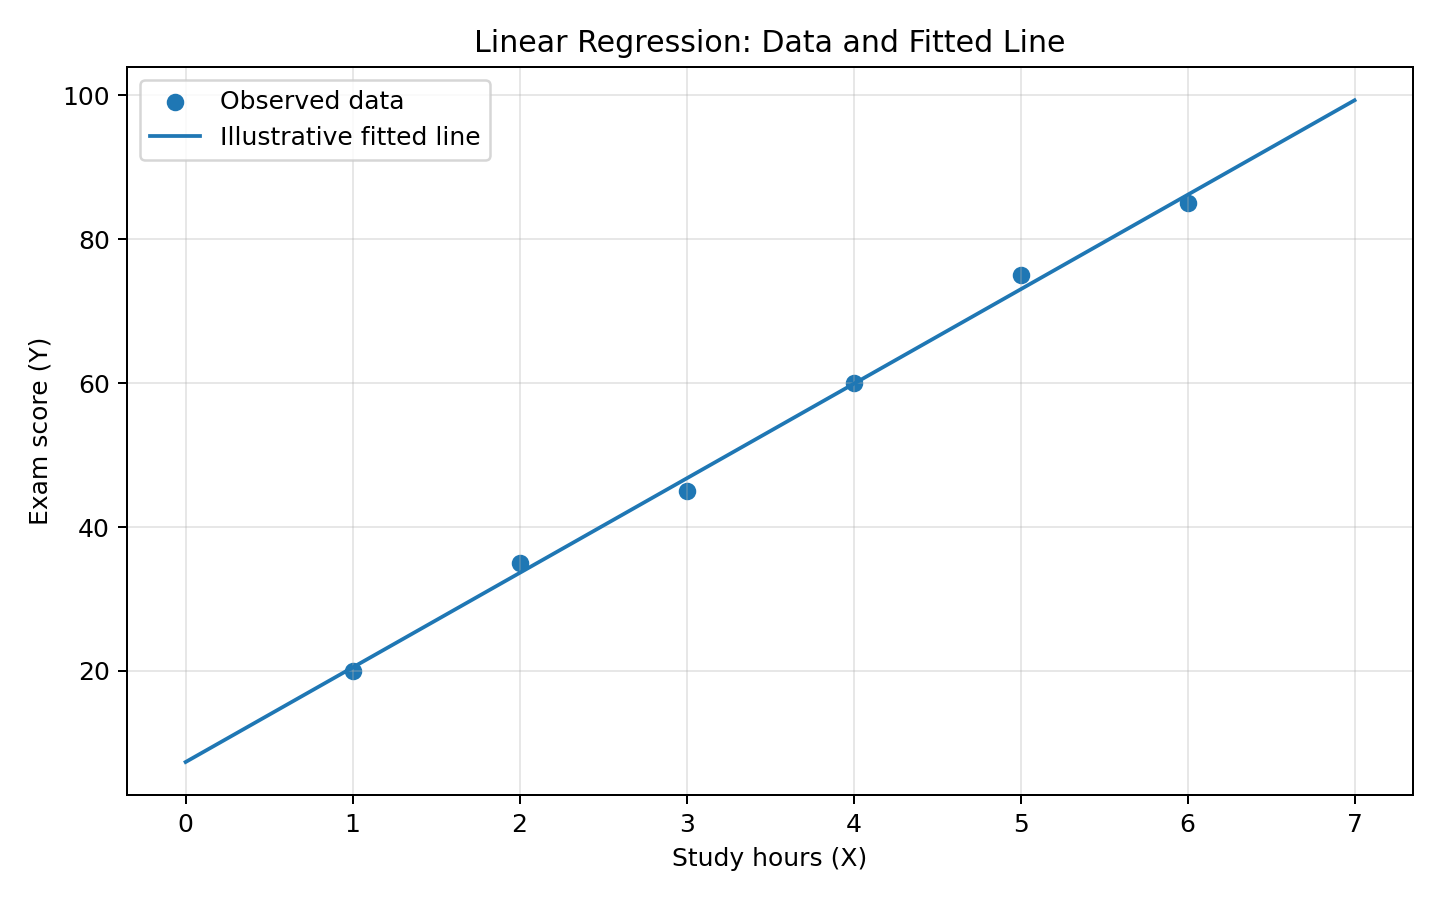
\includegraphics[width=.78\textwidth]{images/linear_regression_fit.png}
\caption{Observed data and an illustrative fitted regression line.}
\end{figure}

The line does not need to pass through every observed point. It aims to fit the overall pattern as well as possible.

\subsection{Important terminology}

\begin{description}
\item[Supervised learning] Training with examples that include known correct outputs.
\item[Feature ($X$)] An input variable used to make a prediction.
\item[Target ($Y$)] The observed output we want to predict.
\item[Regression] Predicting a continuous numerical quantity.
\item[Model] A mathematical function that maps input values to predictions.
\end{description}

\section{The Linear Regression Equation}

For simple linear regression with one feature, the prediction equation is
\[
\boxed{\hat{y}=\beta_0+\beta_1x.}
\]
This has the same mathematical structure as the school equation $y=mx+c$.

\begin{itemize}
\item $x$ is the input feature.
\item $\hat y$ is the predicted output.
\item $\beta_0$ is the intercept.
\item $\beta_1$ is the slope or coefficient.
\end{itemize}

\subsection{The intercept ($\beta_0$)}

The intercept is the model's predicted output when the input is zero:
\[
\hat y\big|_{x=0}=\beta_0.
\]
For example, in $\hat y=10+12x$, the intercept is $10$. The model predicts $10$ when $x=0$. Whether that prediction has a meaningful real-world interpretation depends on the problem and the range of the data.

\subsection{The slope ($\beta_1$)}

The slope describes the change in predicted output for a one-unit increase in the input:
\[
\Delta \hat y = \beta_1 \Delta x.
\]
If $\beta_1=12$, increasing study time by one hour increases the model's predicted score by 12 points. This describes the model's prediction, not necessarily a causal effect.

\subsection{Positive, negative, and zero slopes}

\begin{figure}[H]
\centering
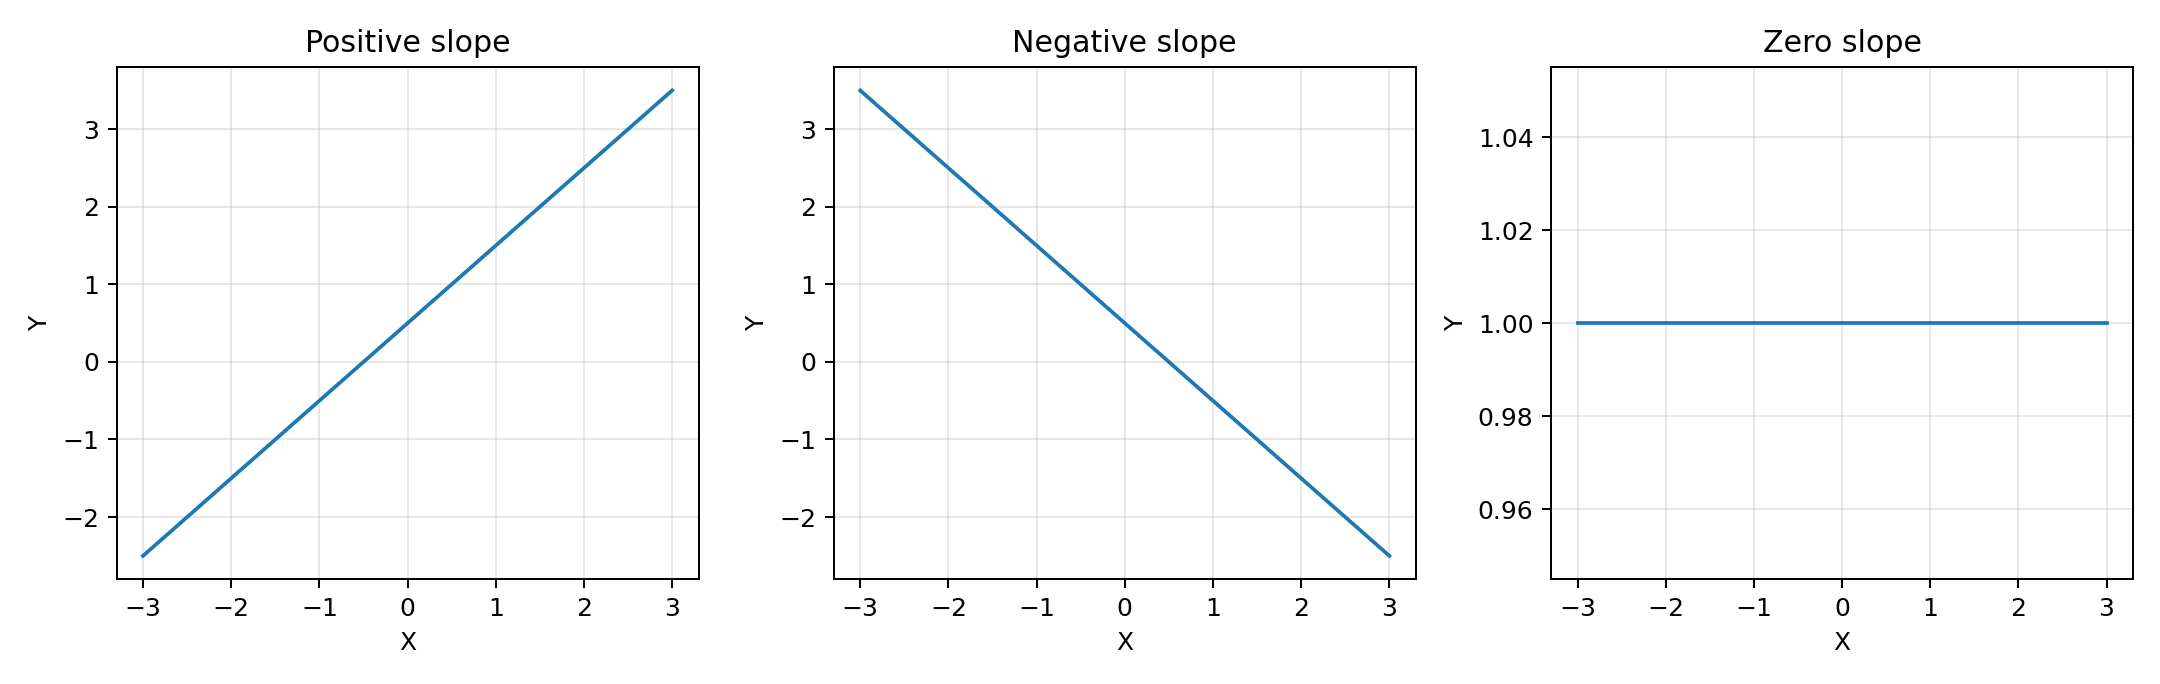
\includegraphics[width=.95\textwidth]{images/slope_types.png}
\caption{Positive, negative, and zero slope examples.}
\end{figure}

\begin{itemize}
\item $\beta_1>0$: predicted $Y$ increases as $X$ increases.
\item $\beta_1<0$: predicted $Y$ decreases as $X$ increases.
\item $\beta_1=0$: the prediction does not change with $X$.
\end{itemize}

\subsection{Worked prediction}

Suppose
\[
\hat y=15+10x.
\]
For a student who studies for six hours,
\[
\hat y=15+10(6)=\boxed{75}.
\]

\subsection{Beta versus beta-hat}

In statistical notation, $\beta_0$ and $\beta_1$ often represent unknown population parameters. Their estimates, calculated from a sample, are written as $\hat\beta_0$ and $\hat\beta_1$. Thus, the fitted model can be written
\[
\hat y=\hat\beta_0+\hat\beta_1x.
\]
Likewise, $y$ is an observed value, while $\hat y$ is a model prediction.

\section{How Does Linear Regression Learn?}

A model makes predictions using its current parameters. We compare those predictions with the actual observations to measure how well the model is performing.

\subsection{Actual values and predictions}

Consider the following data and a deliberately imperfect model:
\[
\hat y=10+10x.
\]

\begin{center}
\begin{tabular}{rrrr}
\toprule
$X$ & Actual $Y$ & Predicted $\hat Y$ & Residual $e=Y-\hat Y$\\
\midrule
1 & 25 & 20 & 5\\
2 & 40 & 30 & 10\\
3 & 50 & 40 & 10\\
4 & 65 & 50 & 15\\
5 & 75 & 60 & 15\\
\bottomrule
\end{tabular}
\end{center}

\subsection{Residuals}

A residual is the difference between an observed value and its prediction:
\[
\boxed{e_i=y_i-\hat y_i.}
\]
A positive residual means the prediction is below the actual value (underprediction). A negative residual means the prediction is above the actual value (overprediction).

\begin{figure}[H]
\centering
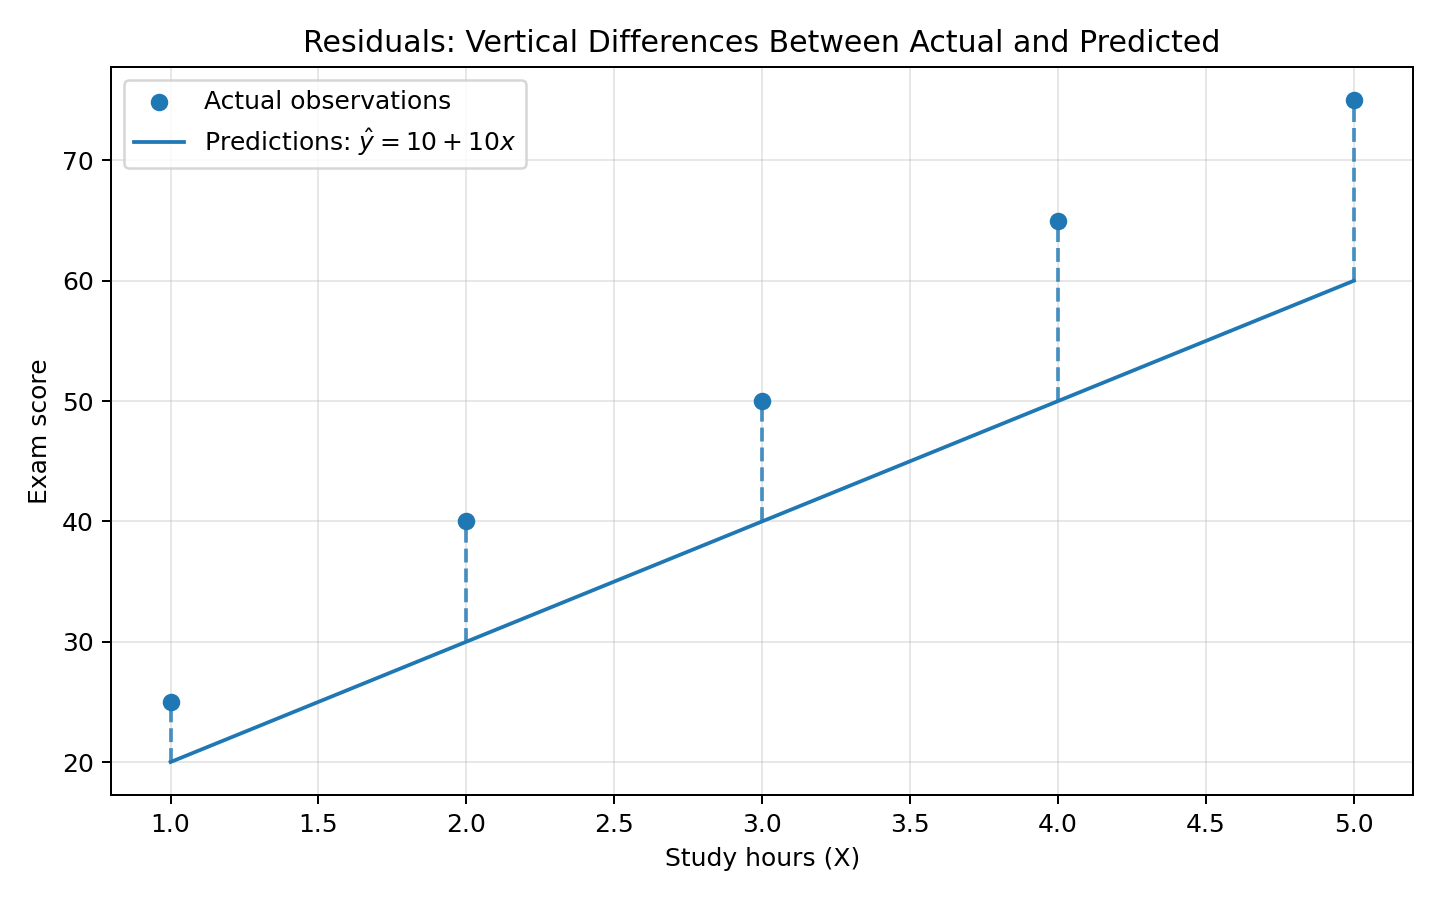
\includegraphics[width=.78\textwidth]{images/residuals.png}
\caption{Residuals are vertical distances between observations and predictions.}
\end{figure}

\subsection{Why not simply sum the residuals?}

Positive and negative residuals can cancel. For example,
\[
5+10-5-10=0.
\]
A sum of zero does not mean every prediction is correct. We therefore use a measure that avoids this cancellation.

\section{Cost Functions: RSS and MSE}

\subsection{Residual Sum of Squares (RSS)}

Square each residual and add the results:
\[
\boxed{RSS=\sum_{i=1}^{n}(y_i-\hat y_i)^2.}
\]
For residuals $[5,10,-5,-10]$,
\[
RSS=5^2+10^2+(-5)^2+(-10)^2=250.
\]
Squaring prevents positive and negative residuals from cancelling and gives larger errors more weight.

\subsection{Mean Squared Error (MSE)}

MSE is the average squared residual:
\[
\boxed{MSE=\frac{1}{n}\sum_{i=1}^{n}(y_i-\hat y_i)^2.}
\]
For the five-observation example, residuals are $[5,10,10,15,15]$:
\[
MSE=\frac{5^2+10^2+10^2+15^2+15^2}{5}
=\frac{675}{5}=\boxed{135}.
\]
For models evaluated on the same target data and scale, a lower MSE means a smaller average squared prediction error.

\subsection{The objective of Linear Regression}

Substitute the prediction equation $\hat y_i=\beta_0+\beta_1x_i$ into MSE. Define the cost function:
\[
\boxed{
J(\beta_0,\beta_1)=
\frac{1}{n}\sum_{i=1}^{n}
(y_i-\beta_0-\beta_1x_i)^2.
}
\]
The learning objective is to find parameter values that minimize this function:
\[
\boxed{\min_{\beta_0,\beta_1}J(\beta_0,\beta_1).}
\]
The cost function gives us a numerical way to compare candidate parameter values.

\section{Gradient Descent: The Main Idea}

Gradient Descent is an optimization algorithm that repeatedly adjusts model parameters in a direction that reduces the cost function.

A useful analogy is walking downhill in fog. At each position, estimate the local downhill direction, take a step, and repeat. In optimization, the cost is analogous to height, the parameters are the position, and the negative gradient gives the steepest local direction of decrease.

\subsection{The loss landscape}

For a one-parameter example, consider
\[
J(\theta)=(\theta-2)^2+1.
\]
The cost is smallest at $\theta=2$. Gradient Descent attempts to approach that minimum through repeated updates.

\begin{figure}[H]
\centering
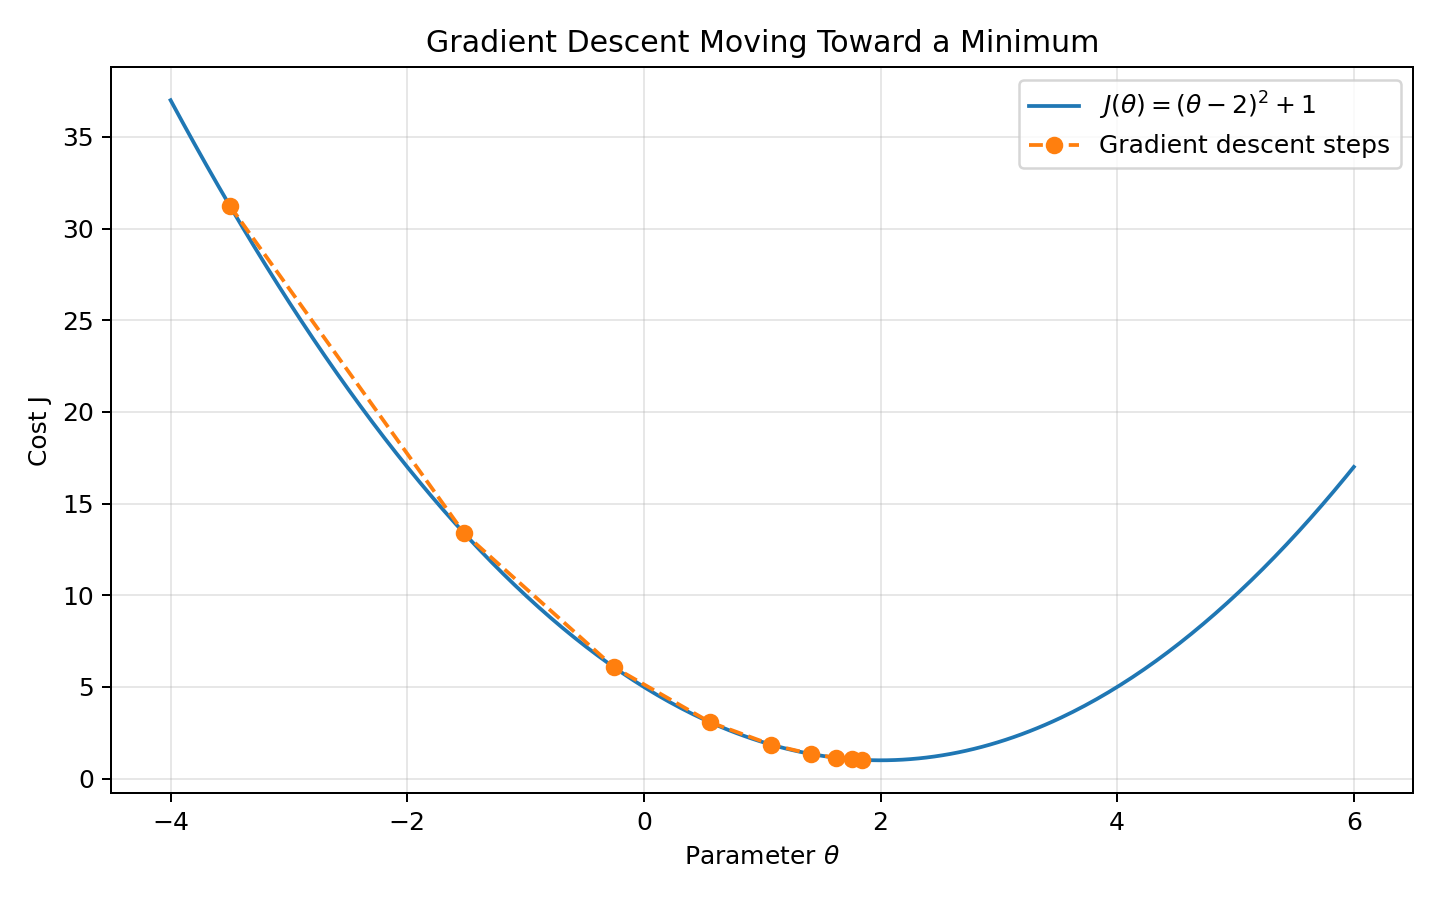
\includegraphics[width=.78\textwidth]{images/gradient_descent_steps.png}
\caption{Illustration of iterative steps moving toward a cost minimum.}
\end{figure}

\subsection{What is a gradient?}

For a single-variable function, the derivative describes the rate at which the function changes:
\[
f(x)=x^2,\qquad \frac{df}{dx}=2x.
\]
For this function:
\begin{itemize}
\item If $x<0$, the derivative is negative.
\item If $x>0$, the derivative is positive.
\item At $x=0$, the derivative is zero.
\end{itemize}
A gradient points in the direction of steepest increase. The negative gradient points in the direction of steepest local decrease.

\subsection{The update rule}

The general Gradient Descent update is
\[
\boxed{
\theta_{\text{new}}=
\theta_{\text{old}}-\alpha
\frac{\partial J}{\partial\theta}.
}
\]
Here $\theta$ is a parameter, $J$ is the cost function, and $\alpha$ is the learning rate. The learning rate controls the step size.

\subsection{Learning rate}

\begin{figure}[H]
\centering
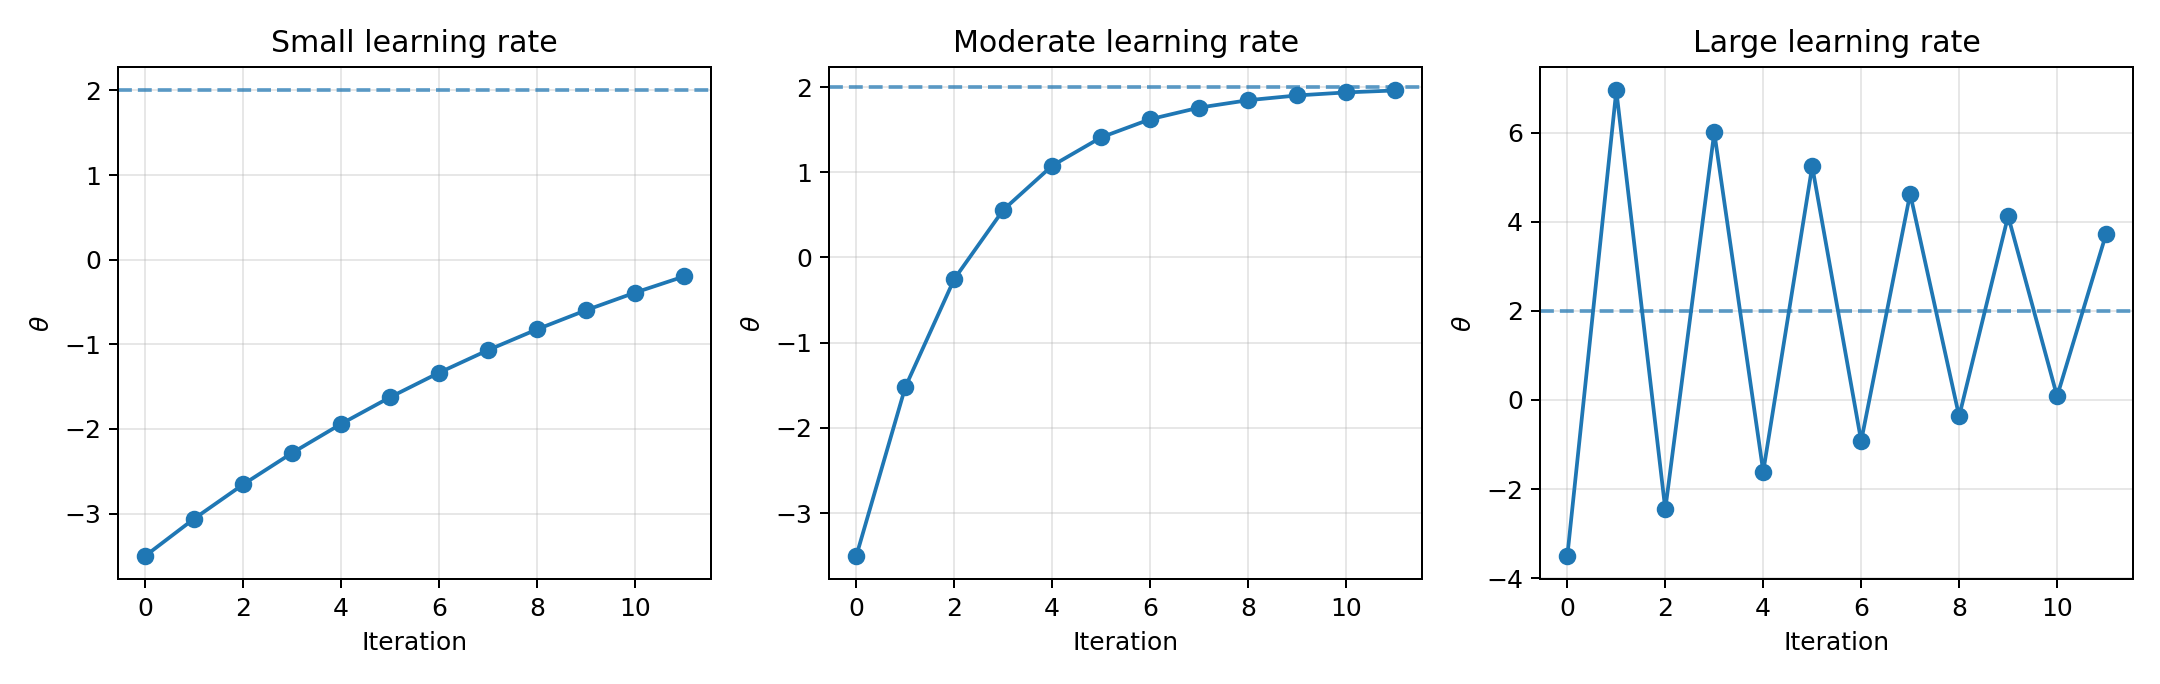
\includegraphics[width=.95\textwidth]{images/learning_rate_comparison.png}
\caption{Illustrative parameter trajectories for different learning rates.}
\end{figure}

\begin{itemize}
\item A learning rate that is too small can make progress very slow.
\item A suitable learning rate can approach the minimum efficiently.
\item A learning rate that is too large can overshoot the minimum or diverge.
\end{itemize}
A value such as $\alpha=0.01$ may be a starting point in some problems, but there is no universally best learning rate.

\section{Gradient Descent for Simple Linear Regression}

Recall the model:
\[
\hat y_i=\beta_0+\beta_1x_i.
\]
Use the MSE cost:
\[
J(\beta_0,\beta_1)=
\frac{1}{n}\sum_{i=1}^{n}
(y_i-\beta_0-\beta_1x_i)^2.
\]

The partial derivatives are
\[
\boxed{
\frac{\partial J}{\partial\beta_0}
=\frac{2}{n}\sum_{i=1}^{n}(\hat y_i-y_i)
}
\]
and
\[
\boxed{
\frac{\partial J}{\partial\beta_1}
=\frac{2}{n}\sum_{i=1}^{n}(\hat y_i-y_i)x_i.
}
\]

The parameters are updated as follows:
\[
\boxed{
\beta_0\leftarrow\beta_0-
\alpha\frac{\partial J}{\partial\beta_0}
}
\]
\[
\boxed{
\beta_1\leftarrow\beta_1-
\alpha\frac{\partial J}{\partial\beta_1}.
}
\]
Both gradients should be calculated using the current parameter values before either parameter is updated.

\section{One Complete Numerical Update}

Suppose we have one observation:
\[
x=2,\qquad y=6.
\]
Start with
\[
\beta_0=0,\qquad \beta_1=1,\qquad \alpha=0.1.
\]

\subsection*{Step 1: Prediction}
\[
\hat y=\beta_0+\beta_1x=0+1(2)=2.
\]

\subsection*{Step 2: Gradients}
For one observation, $n=1$:
\[
\frac{\partial J}{\partial\beta_0}
=2(\hat y-y)=2(2-6)=-8,
\]
\[
\frac{\partial J}{\partial\beta_1}
=2(\hat y-y)x=2(2-6)(2)=-16.
\]

\subsection*{Step 3: Update the intercept}
\[
\beta_0=0-0.1(-8)=\boxed{0.8}.
\]

\subsection*{Step 4: Update the slope}
\[
\beta_1=1-0.1(-16)=\boxed{2.6}.
\]

The updated model is
\[
\hat y=0.8+2.6x.
\]
For $x=2$:
\[
\hat y=0.8+2.6(2)=6.
\]
The initial squared error was $(6-2)^2=16$, while the updated squared error is $(6-6)^2=0$. This simple one-observation example reaches the target exactly after one update; real datasets generally require many updates and will not fit perfectly.

\section{Iterations and Convergence}

One iteration is one complete parameter update. A typical Gradient Descent iteration does the following:
\begin{enumerate}
\item Calculate predictions using the current parameters.
\item Calculate the cost.
\item Calculate the gradients.
\item Update the parameters.
\item Repeat.
\end{enumerate}

The process may stop when the cost changes very little, the gradient becomes sufficiently small, or a chosen maximum number of iterations is reached. This is called a stopping criterion. Convergence does not automatically guarantee good performance on unseen data; model evaluation is still necessary.

\section{Summary: The Complete Learning Pipeline}

\begin{enumerate}
\item Start with training data containing features $X$ and targets $Y$.
\item Initialize $\beta_0$ and $\beta_1$.
\item Predict with $\hat y=\beta_0+\beta_1x$.
\item Calculate residuals $e_i=y_i-\hat y_i$.
\item Calculate the cost using MSE.
\item Calculate the partial derivatives of the cost.
\item Update $\beta_0$ and $\beta_1$ using the learning rate.
\item Repeat until the stopping condition is met.
\item Evaluate the fitted model on data not used for training.
\end{enumerate}

\section{Key Formula Sheet}

\begin{align*}
\text{Prediction:}\quad & \hat y=\beta_0+\beta_1x\\[4pt]
\text{Residual:}\quad & e_i=y_i-\hat y_i\\[4pt]
\text{RSS:}\quad & RSS=\sum_{i=1}^{n}(y_i-\hat y_i)^2\\[4pt]
\text{MSE:}\quad & J=\frac{1}{n}\sum_{i=1}^{n}(y_i-\hat y_i)^2\\[4pt]
\text{Intercept gradient:}\quad &
\frac{\partial J}{\partial\beta_0}
=\frac{2}{n}\sum_{i=1}^{n}(\hat y_i-y_i)\\[4pt]
\text{Slope gradient:}\quad &
\frac{\partial J}{\partial\beta_1}
=\frac{2}{n}\sum_{i=1}^{n}(\hat y_i-y_i)x_i\\[4pt]
\text{Gradient Descent:}\quad &
\theta\leftarrow\theta-\alpha\frac{\partial J}{\partial\theta}
\end{align*}

\textbf{Next learning milestone:} Derive the two partial derivatives step by step using the chain rule, then implement Linear Regression from scratch in Python and NumPy without using \texttt{scikit-learn}.

\end{document}
